%-------------------------------------------------%
% 2025-04-01 - Emerson Ribeiro de Mello - mello@ifsc.edu.br
%-------------------------------------------------%
% Sets aspect ratio to 16:9, and frame size to 160 mm by 90 mm.
\documentclass[aspectratio=169]{beamer}

% Sets aspect ratio to 4:3, and frame size to 128 mm by 96 mm
% \documentclass{beamer}

% Sets aspect ratio to 16:10, and frame size to 160 mm by 100 mm.
% \documentclass[aspectratio=161]{beamer}

\usepackage[english,brazil]{babel}


\usepackage[style=abnt,noslsn,justify]{biblatex}
\renewcommand*{\bibfont}{\small}
\usepackage{csquotes}
\addbibresource{referencias.bib}

% \pgfdeclareimage[width=3cm]{ifsclogo}{img/ifsc-logo-h-branco.png}


% Crie cores personalizadas para usar no tema
\definecolor[named]{novaCor}{HTML}{303A52}
\definecolor{verdeescuro}{RGB}{0,112,19}

% Outras cores já definidas no tema
% redwine
% azulcinza
% azulescuro
% cyanIFSC
% fundoIFSC
% cinzaescuro
% verdeifsc
% vermelhoifsc
% vermelhoifscclaro

% Theme parameters
\usetheme[
    % foreground=redwine, % cor do texto (usado no título dos slides) 
    % background=white, % cor do fundo dos slides
    % textfg=black, % cor do texto nos slides
    % titlefg=redwine, % cor do texto do slide de título
    % titlebg=white, % cor do fundo do slide de título
    % frametitlefg=white, % cor do texto do título do frame
    % frametitlebg=redwine, % cor do fundo do título do frame
    % sectionfg=redwine, % cor do texto do slide da seção
    % sectionbg=white, % cor do fundo do slide de seção
    % blocktitlefg=white, % cor do texto do título dos blocos
    % blocktitlebg=redwine, % cor do fundo do título dos blocos
    % blockbodyfg=cinzaescuro, % cor do texto dentro dos blocos
    % itemsep=7pt % Espaçamento entre os itens das listas 
]{ifsclean}



% -------------------------------------------------%
%              Título 
% -------------------------------------------------%
\title{Título da apresentação}

\subtitle{Modelo de slides para o IFSC}

\author{Emerson Ribeiro de Mello}

\institute{mello@ifsc.edu.br}

% \date{}


%-------------------------------------------------%
\begin{document}
% -------------------------------------------------%

\begin{frame}[plain, noframenumbering]
    \maketitle
\end{frame}

\begin{frame}[plain, noframenumbering]{Licenciamento}
    \licenciamentoLivre
\end{frame}

\begin{frame}[plain, noframenumbering]{Agenda}
    \tableofcontents
\end{frame}
% -------------------------------------------------%


\section{Listas}


\begin{frame}{Lista de itens}
    \begin{enumerate}
        \item Primeiro item
        \begin{itemize}
            \item \Myhref{https://emersonmello.me}{Aqui tem um exemplo de \textit{link} para um \textit{site} usando o comando \texttt{Myhref}}
            \item Segundo item
        \end{itemize}
        \item Segundo item
        \item Terceiro item 
        \begin{itemize}
            \item Neste linha é apresentado um item que tem um texto grande que deverá ocupar mais de uma linha no slide. Assim, espera-se mostrar como será o alinhamento na margem esquerda
            \item Segundo item
        \end{itemize}
    \end{enumerate}
\end{frame}

\subsection{Animações}

\begin{frame}{Animação com lista de itens}
\begin{itemize}[<+->]
    \item\only<1>{Eu não sei quem criou o~\TeX}\only<2->{\st{Eu não sei quem criou o~\TeX}} 
    \item O~\TeX~foi criado por Donald Knuth
    \begin{itemize}
        \item<.-> O~\TeX~é um sistema de tipografia 
    \end{itemize}
    \item Leslie Lamport criou o~\LaTeX~\cite{lamport94}
    \begin{itemize}
        \item<.-> O~\LaTeX~é um conjunto de macros para o~\TeX 
    \end{itemize}
    \item Em \textcite{knuth74} temos um dos trabalhos mais importantes de Donald Knuth
    
\end{itemize}
\end{frame}

\begin{frame}{Uso do \texttt{alert}}
    \begin{itemize}
        \item<1-| alert@1> Aparecerá desde do slide 1 e receberá destaque no slide 1
        \item<1-| alert@2> Aparecerá desde do slide 1 e receberá destaque no slide 2
        \item<1-| alert@3> Aparecerá desde do slide 1 e receberá destaque no slide 3
        \item<4-| alert@4> Aparecerá desde do slide 4 e receberá destaque no slide 4
    \end{itemize} 
\end{frame}

\subsection{Colunas}

\begin{frame}{Listas em colunas}
    \begin{columns}[t, onlytextwidth]
        \column{0.5\textwidth}
            \begin{itemize}
                \item Item 1
                \begin{itemize}
                    \item Subitem 1.1
                    \item Subitem 1.2
                \end{itemize}
                \item Item 2
                \item Item 3
            \end{itemize}
        
        \column{0.5\textwidth}
            \begin{enumerate}
                \item First
                \item Second
                \begin{enumerate}
                    \item Sub-first
                    \item Sub-second
                \end{enumerate}
                \item Third
            \end{enumerate}
    \end{columns}
\end{frame}

\begin{frame}{Listas e figuras}
\begin{columns}
    \column{.5\linewidth}
     \begin{center}
        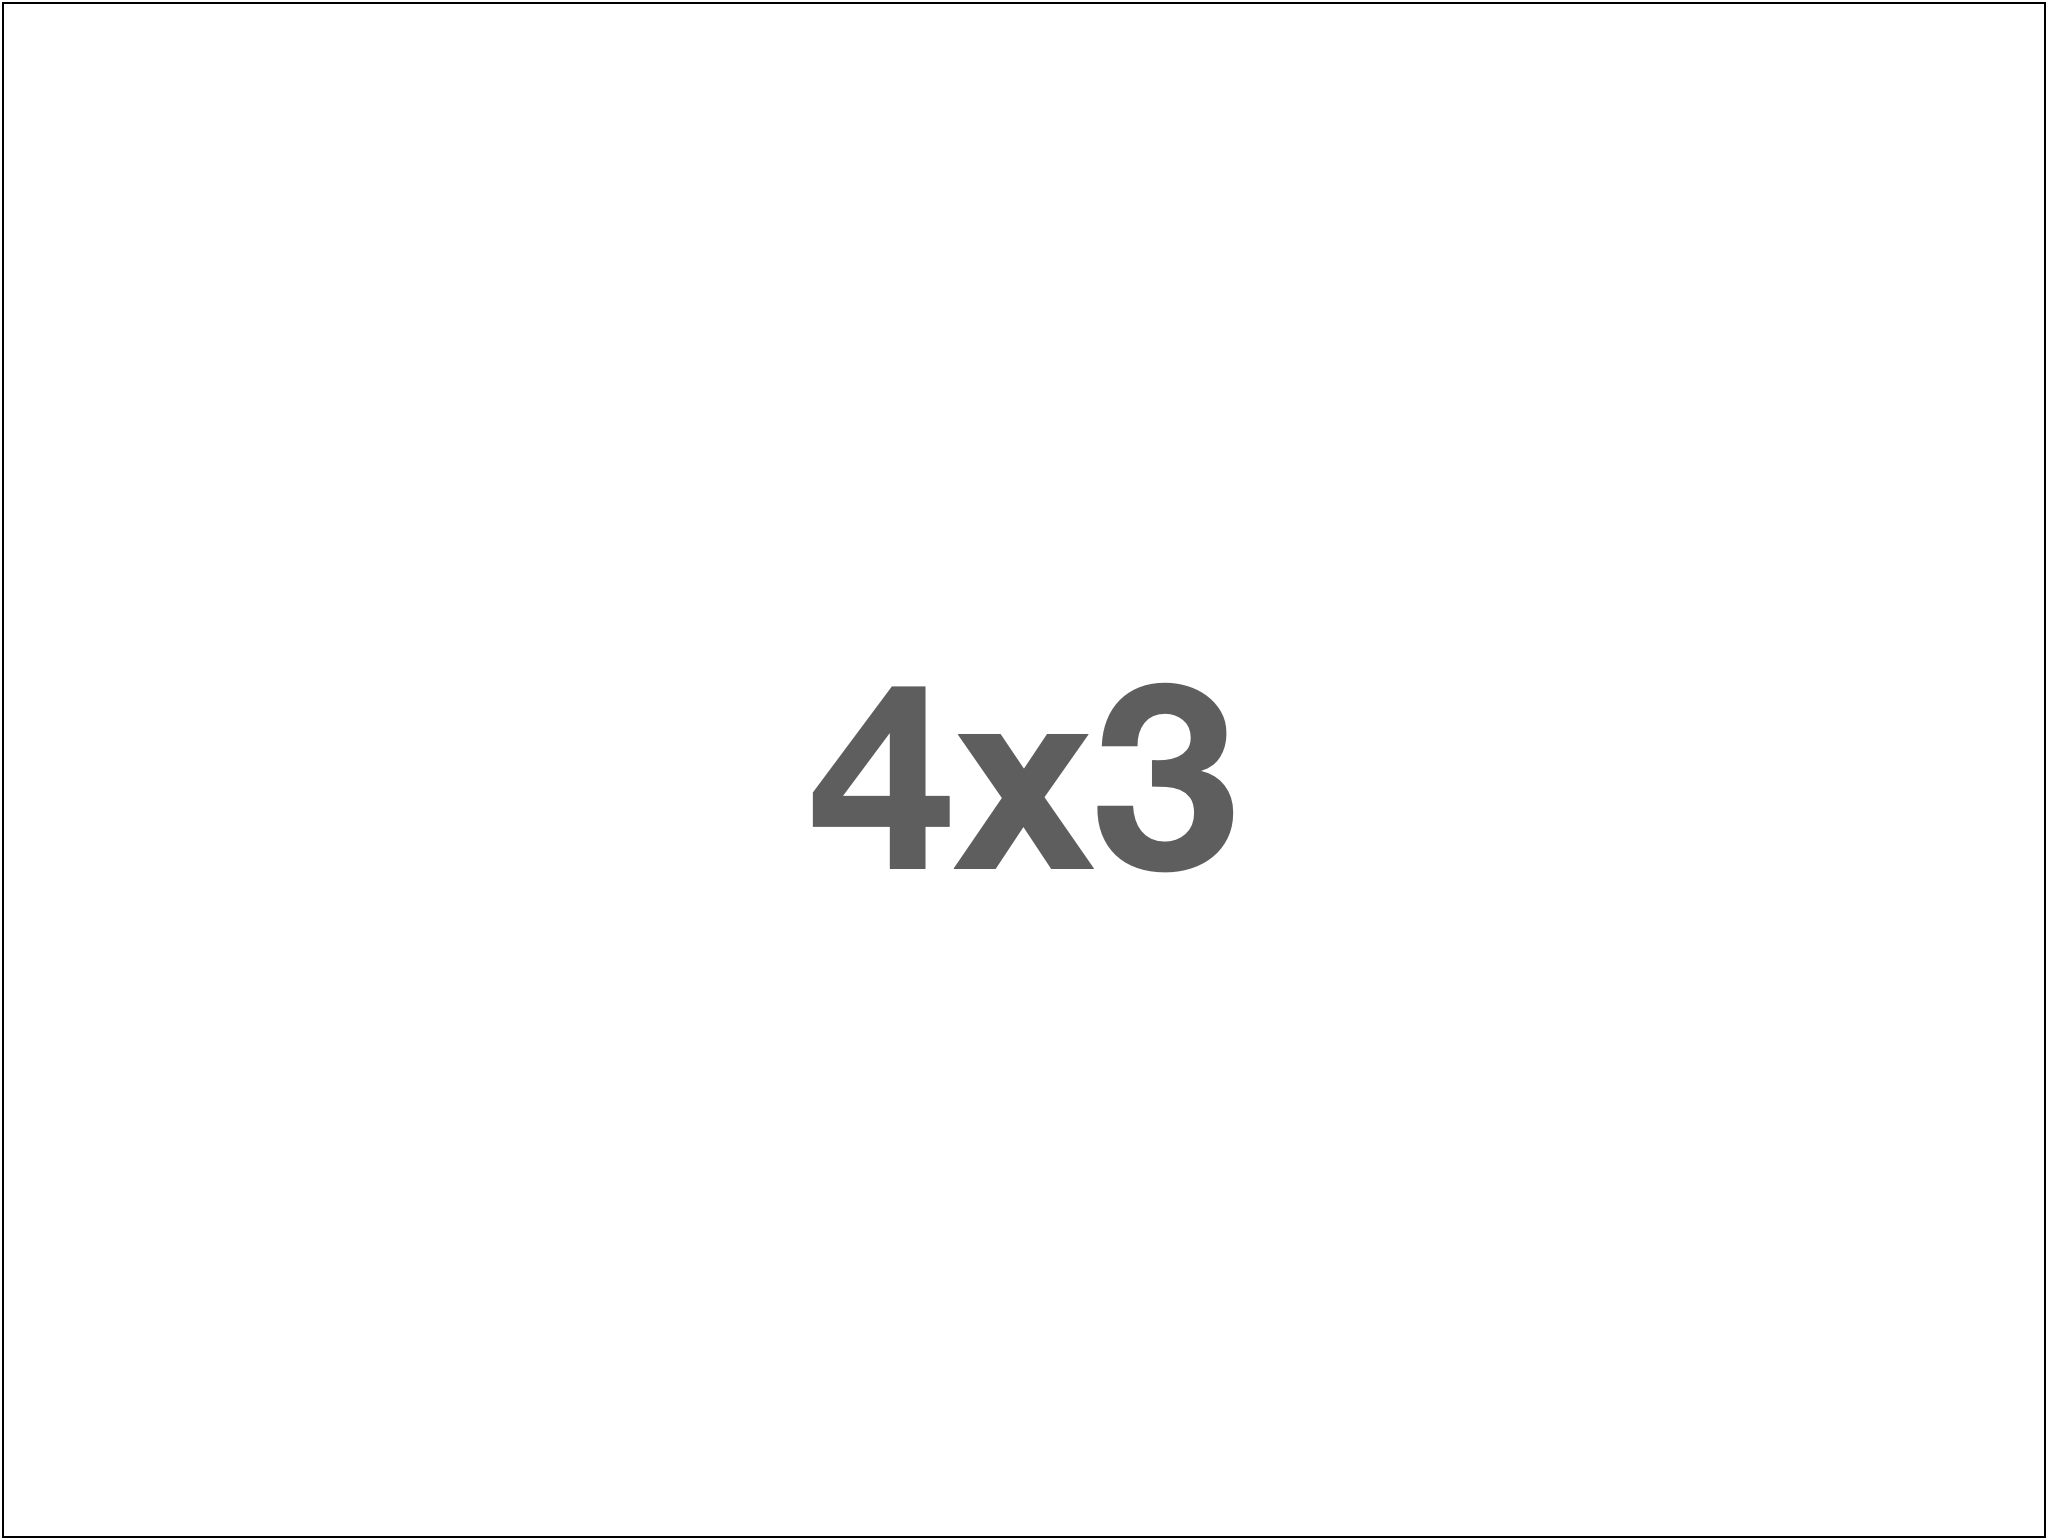
\includegraphics[width=\linewidth]{figs/4x3.png}
     \end{center}
    \column{.5\linewidth}
    \begin{itemize}
        \item Item 1
        \begin{itemize}
            \item Subitem 1.1
            \item Subitem 1.2
        \end{itemize}
        \item Item 2
        \item Item 3
    \end{itemize}
\end{columns} 
\end{frame}


\section{Blocos}


\begin{frame}{Blocos}
    \begin{block}{Esse é um bloco}
        Isso é um teste
    \end{block}
    \begin{block}{}
    Bloco sem título	
    \end{block}
    \begin{alertblock}{Alerta}
        Esse é um alerta
    \end{alertblock}

    \begin{exampleblock}{Exemplo}
        Esse é um exemplo
    \end{exampleblock}
\end{frame}


\begin{frame}{Blocos personalizados}

    \begin{informacao}
    Isso é uma mensagem de informação
    \end{informacao}
    
    \begin{informacaoazul}
        Isso é uma mensagem de informação
    \end{informacaoazul}

    \begin{atencao}
        Isso é uma mensagem de atenção
    \end{atencao}
    
    \begin{cuidado}
        Isso é uma mensagem de cuidado
    \end{cuidado}
\end{frame}

\begin{frame}[allowframebreaks]{Blocos personalizados}{Inspirados nos blocos Markdown do GitHub}
\begin{nota}
    Para apresentar uma informação útil
\end{nota}

\begin{tip}
    Para apresentar uma dica
\end{tip}

\begin{important}
    Informação importante que precisa ser destacada
\end{important}

\begin{warning}
    Algo que precisa ser observado com atenção
\end{warning}

\begin{caution}
    Para chamar a atenção do leitor para algo que pode ser perigoso
\end{caution}
\end{frame}


\begin{frame}{Horários}
    {Veja outros ícones em \url{https://ctan.org/pkg/fontawesome}}
    \begin{itemize}
        \item Horário das aulas 
        \begin{caixa}[azul]{white}{\faCalendar}
            \begin{itemize}
                \item 15:40 -- 17:30 - quarta-feira
                \item 13:30 -- 15:20 - quinta-feira
            \end{itemize}
        \end{caixa}
        \item Atendimento extraclasse
        \begin{caixa}[azul]{white}{\faCalendar}
            \begin{itemize}
                \item 10:00 -- 12:00 - sexta-feira
            \end{itemize}
        \end{caixa}
    \end{itemize}
\end{frame}


\section{Figuras}

\begin{frame}{Figura 4x3}
    \begin{center}
        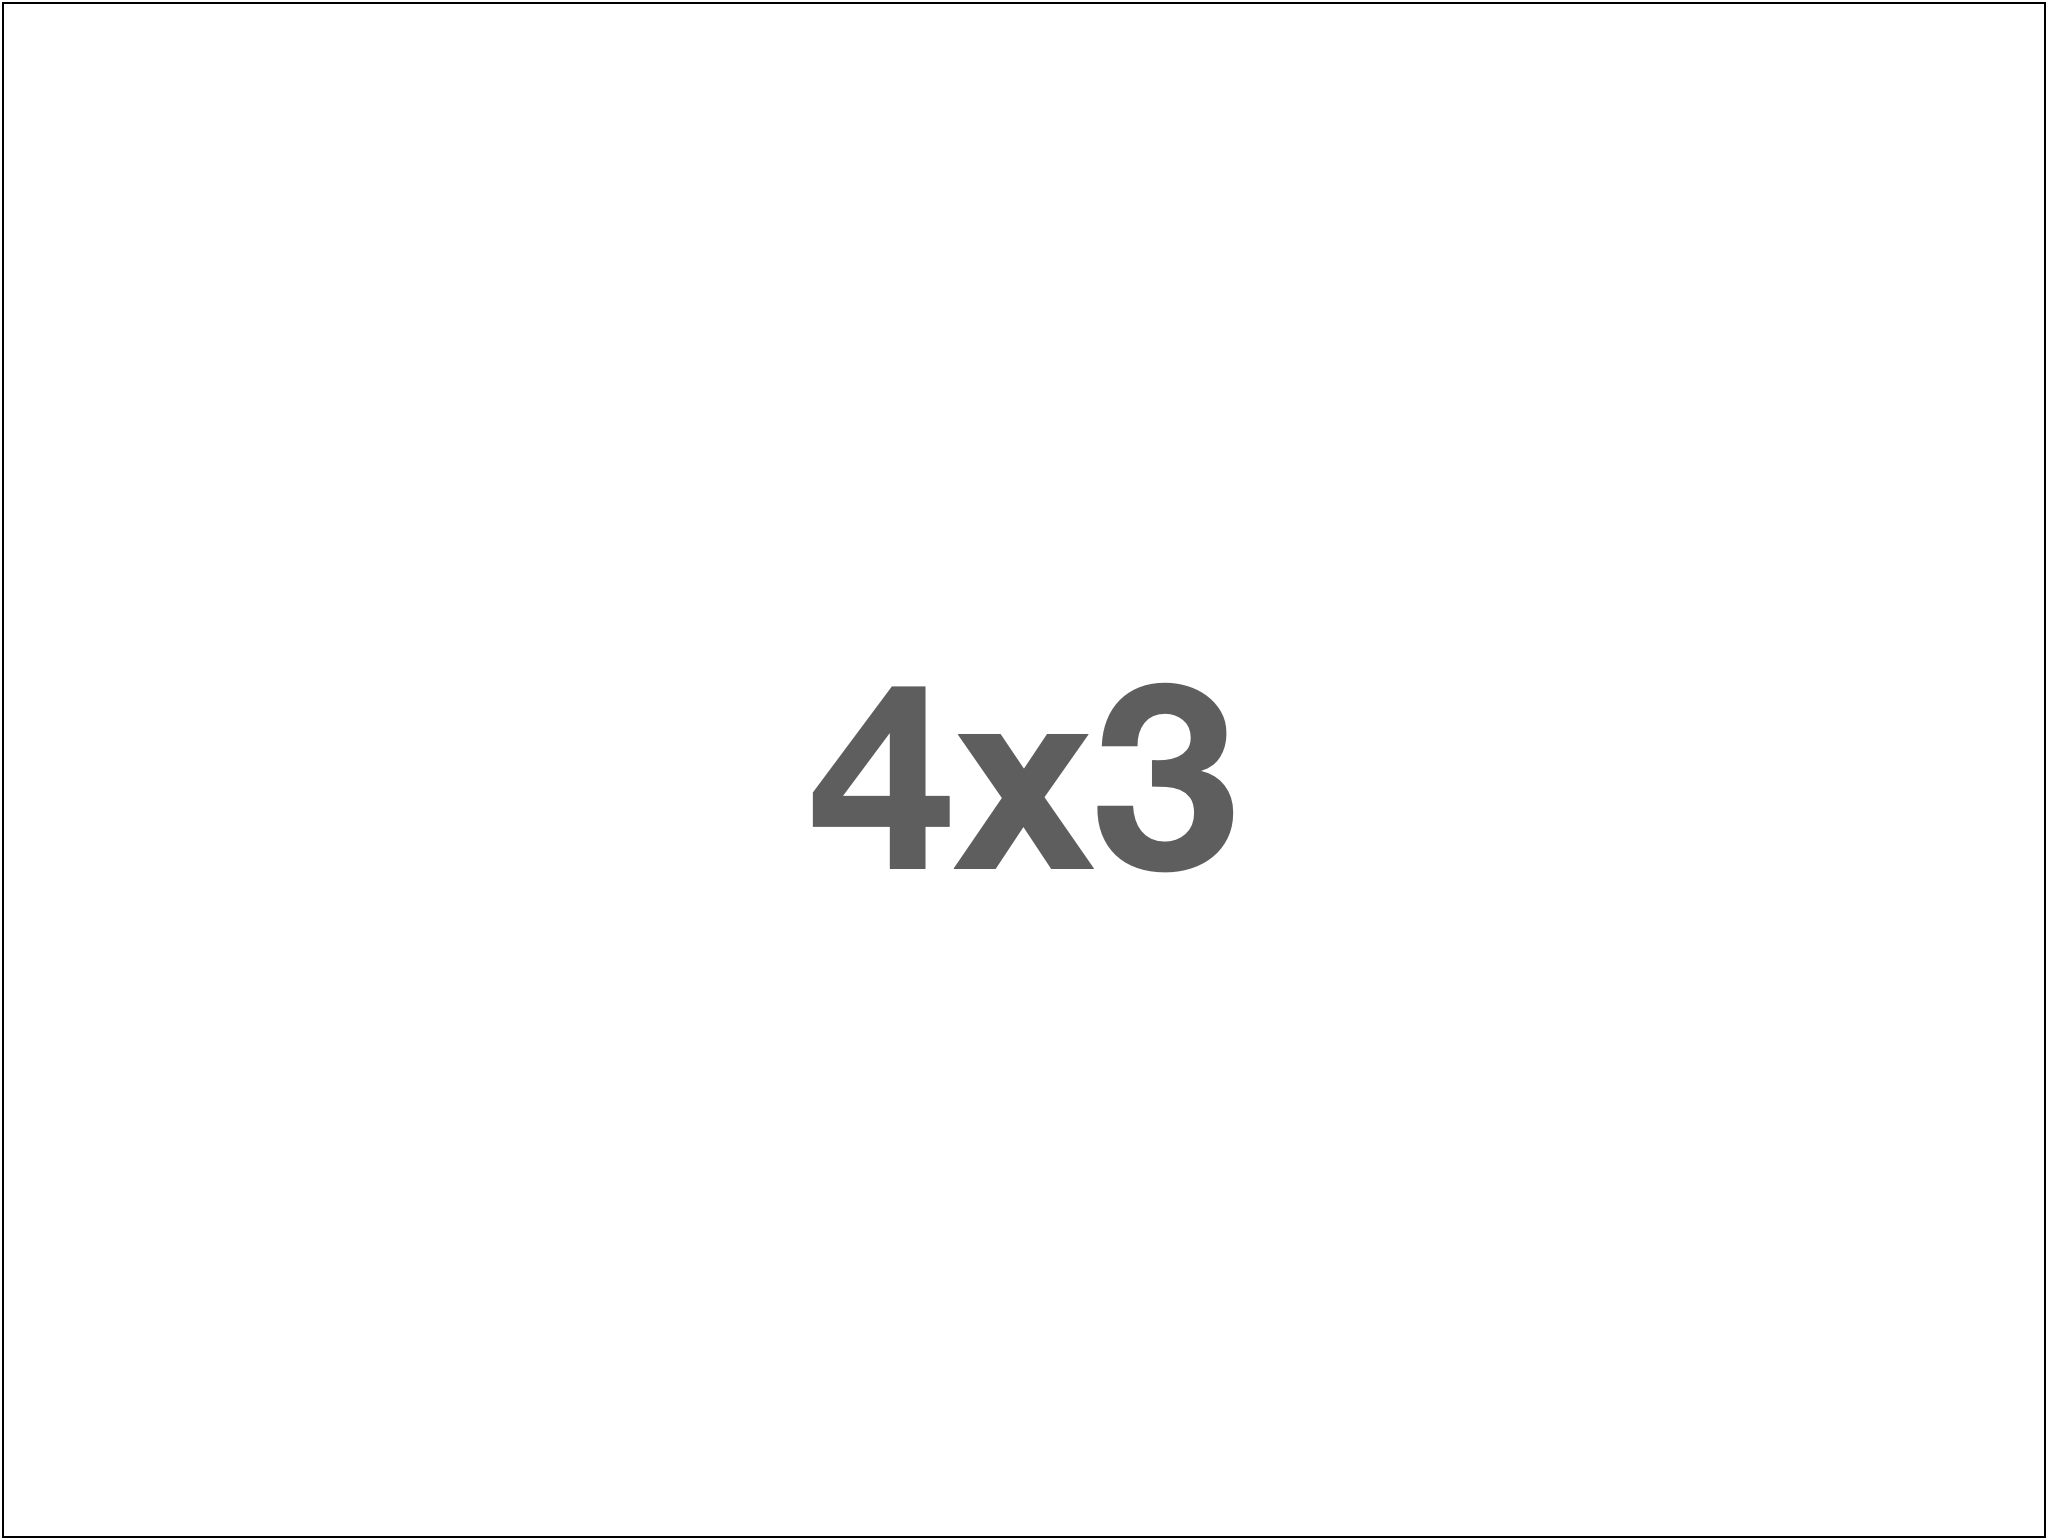
\includegraphics[height=.8\paperheight]{figs/4x3.png}
    \end{center}
\end{frame}
    

\begin{frame}{Figura 16x9}
\begin{center}
    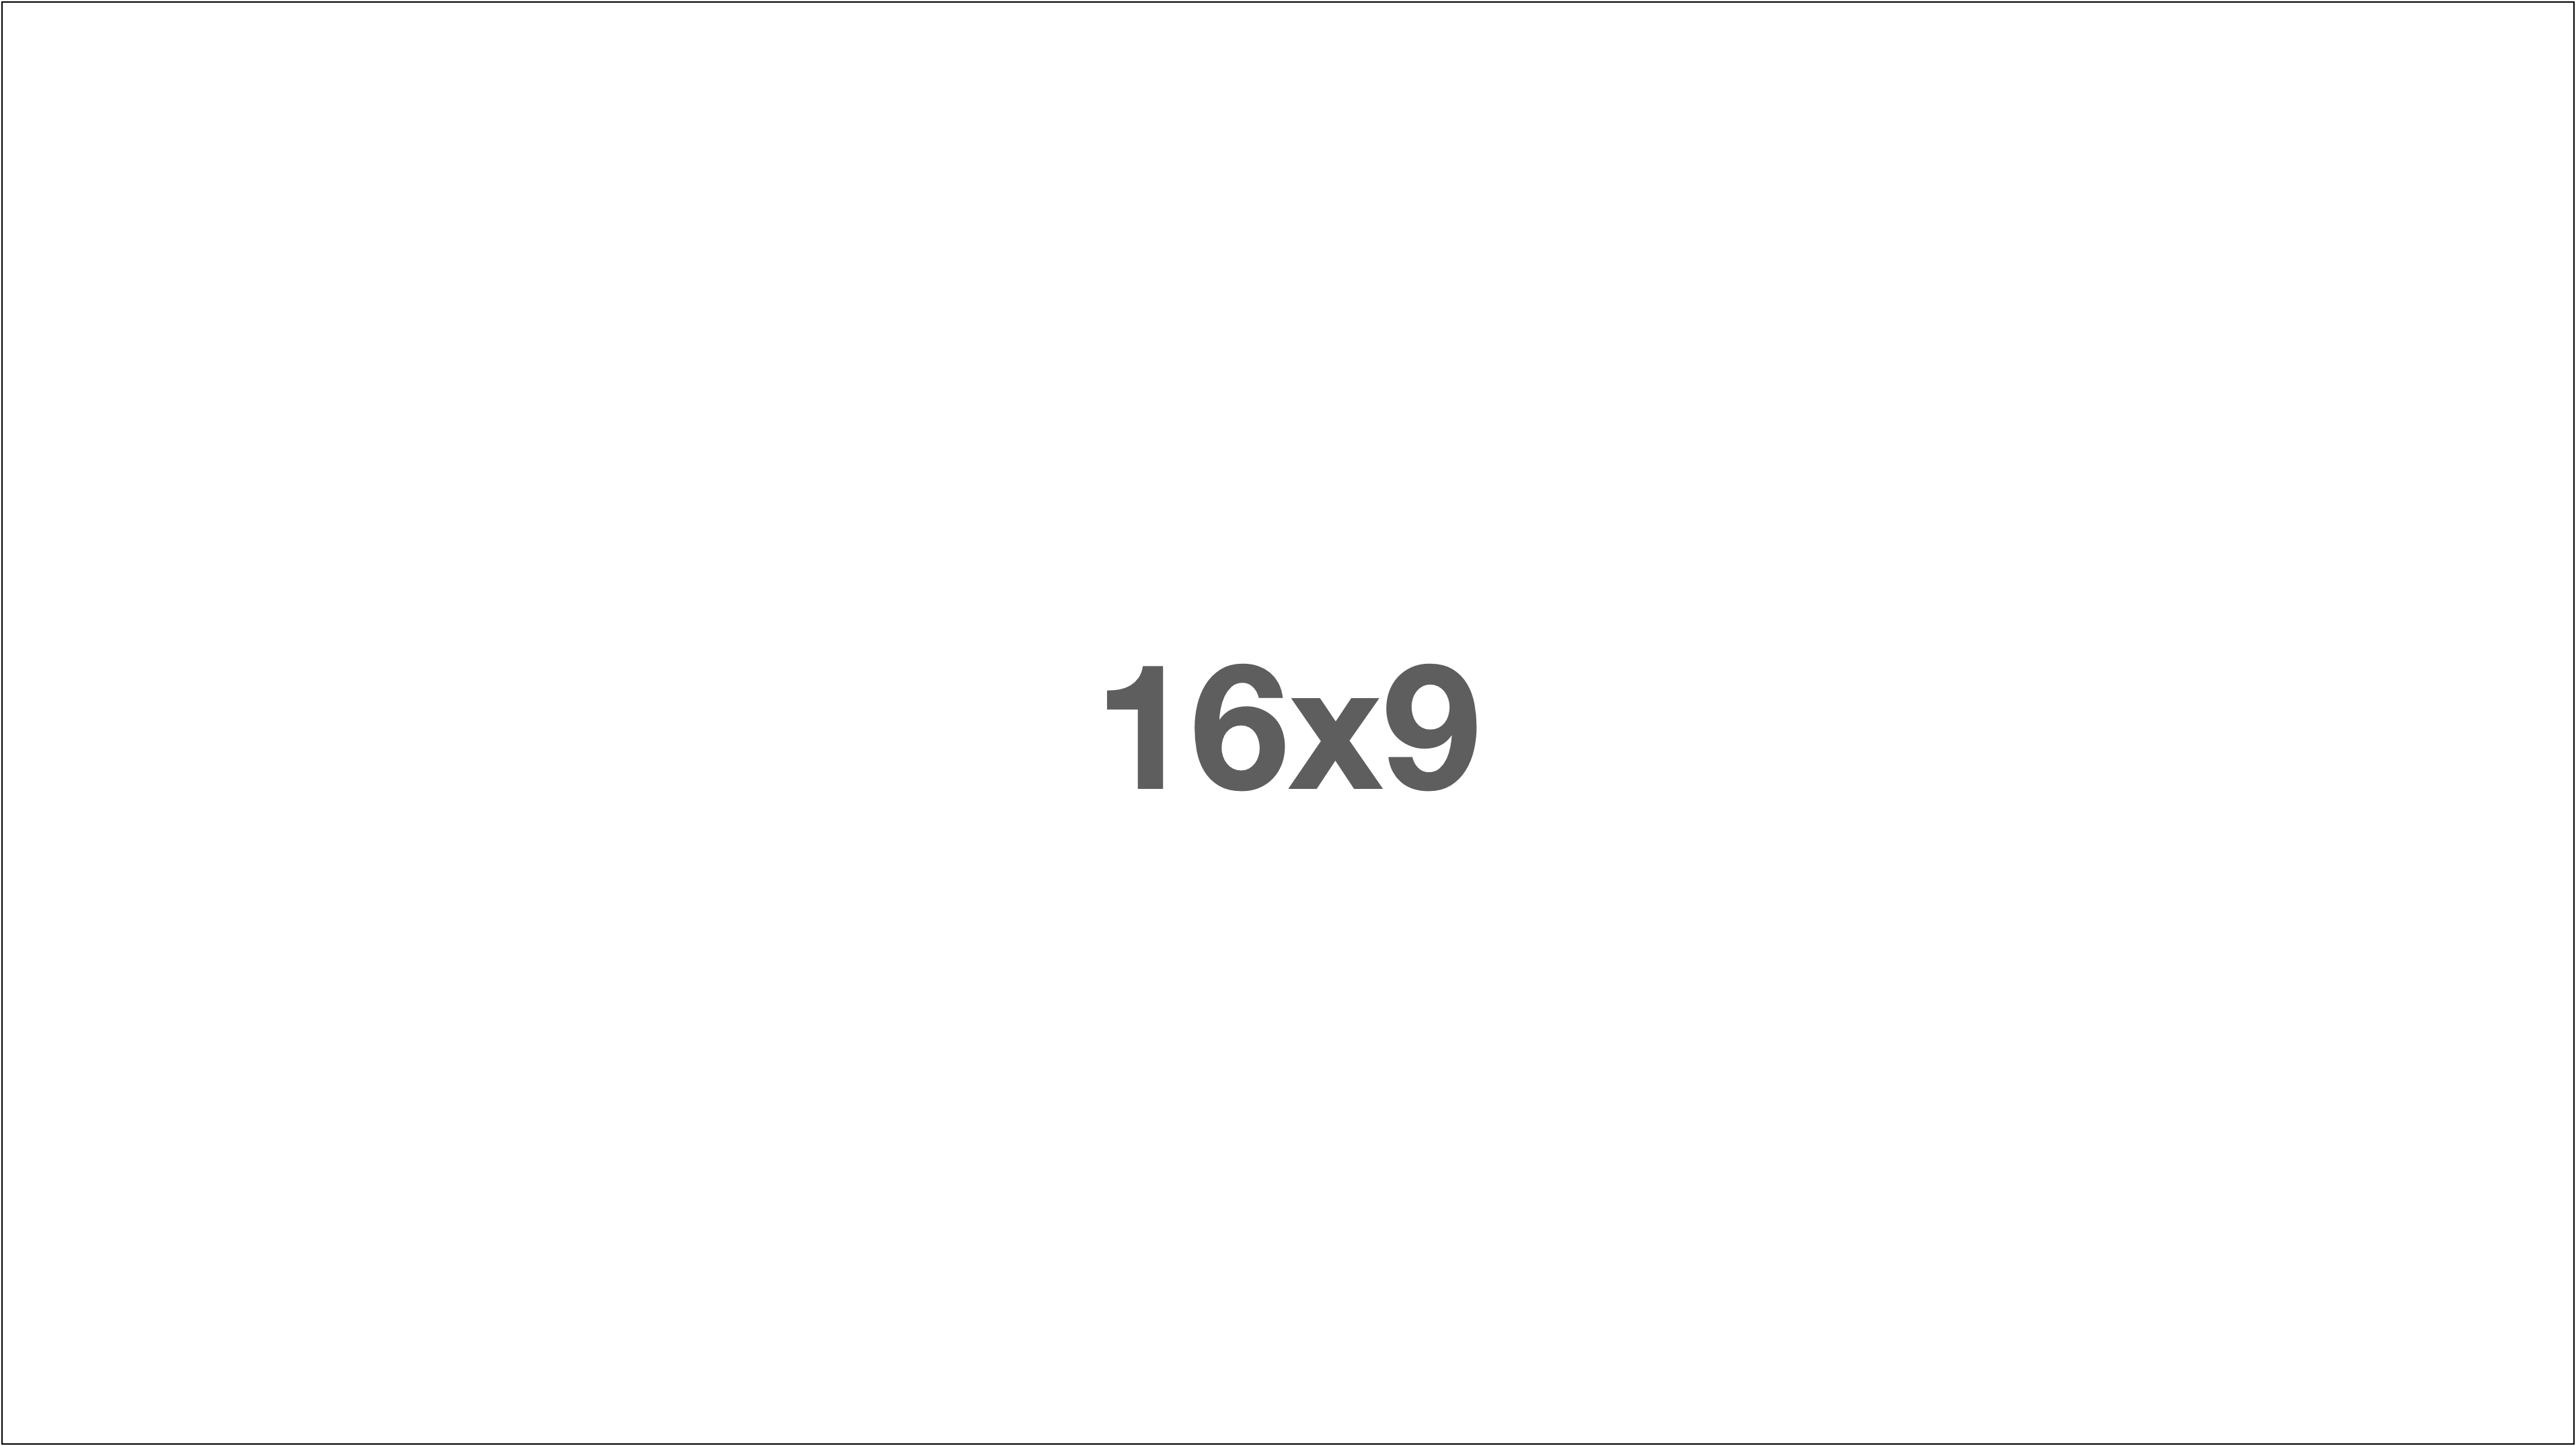
\includegraphics[width=.95\linewidth]{figs/16x9.png}
\end{center}
\end{frame}

\section{Tabelas}

\begin{frame}{Tabelas}
\begin{center}
    \begin{tabular}{l r r}\\\toprule
        Produto & Quantidade & Valor (R\$) \\\midrule
        Água    &      100   &   1,50 \\ 
        Banana  &       10   &   3,00 \\
        Maça    &        1   &   2,50 \\ \bottomrule
    \end{tabular}
\end{center}
\end{frame}

\section{Incluindo código fonte}


\begin{frame}[fragile]{Olá mundo em C}
    \lstinputlisting[style=ansic,caption={Olá mundo},label={cod:olac}]{codigos/olamundo.c}
\end{frame}

\begin{frame}[fragile]{Olá mundo em Java}
\begin{lstlisting}[style=java]
public class App{

    public static void main(String[] args){
        System.out.println("Olá mundo");
    }

}
\end{lstlisting}
\end{frame}

% Para permitir que o código fonte seja quebrado em mais de um slide. Se as referências couberem em um único slide, então pode omitir o uso do allowframebreaks
\begin{frame}[allowframebreaks]{Referências}
    % para incluir todas as referências do arquivo referencias.bib, mesmo sem citá-las explicitamente com os comandos \cite ou \textcite
    \nocite{*}
    \printbibliography
\end{frame}
    
% Se não quiser usar o pacote biblatex, use o seguinte código
% \begin{frame}{Referências}
%     \nocite{*}
%     \bibliography{referencias}
%     \bibliographystyle{plain}
% \end{frame}

\appendix

\section{Slides de backup}

\begin{frame}{Slide de backup}
    \usebeamercolor[fg]{normal text}
    Slides de backup são úteis para incluir materiais adicionais, necessários somente para ajudar a responder possíveis perguntas da plateia
    \vfill
    O pacote \texttt{appendixnumberbeamer} é usado para não numerar os slides de backup
\end{frame}


\end{document}